\originalchapter{文本预测、生成与上下文学习}\label{ch:lm}
\originalsection{文本怎样成为概率对象}\label{sec:lm-tokens}
先把语言模型的任务定义清楚, 再在第 \ref{ch:nn}、\ref{ch:attention} 章构造实现它的计算图. 当前问题是: 给定一段文本, 预测接下来会出现的内容. 网络实际读取整数, 输出实数向量, 因而首先必须约定文本与整数序列之间的映射.

\begin{definition}
固定有限词表 $\mathcal V=\{0,\ldots,V-1\}$. 分词器把文本映为 token 序列, 每个 token 是词表中的一个整数. 解码器把合法 token 序列还原为文本. 本章假定分词规则确定, 词表中有开始符 \texttt{<bos>} 和结束符 \texttt{<eos>}, 并把原始文本里的同名字符串与专用控制符区分.
\end{definition}
Token 不必是完整单词. 汉字、UTF-8 字节、子词和完整词都可以成为单位. 同一字符串 ``cats'' 可以编码为一个单位, 也可以编码为 ``cat'' 与 ``s'' 两个单位. 较大的词表能缩短某些文本, 但会扩大词嵌入和输出矩阵, 并使稀有单位更难估计. 字节词表容易覆盖陌生字符串, 代价是序列可能更长. 这些取舍会同时影响统计任务与计算成本.

BPE 的基本操作可用极小例子理解. 若训练语料中有 ``aaab'' 与 ``aab'', 从字符开始, 第一份的相邻对是 $aa,aa,ab$, 第二份是 $aa,ab$. 对 $aa$ 的计数为 3, 对 $ab$ 的计数为 2, 因而优先把 $aa$ 合成新单位. 从左到右作不重叠合并后, 两份分别成为 $(aa,a,b)$ 与 $(aa,b)$. 下一轮必须重新统计当前单位对, 不能沿用原字符对计数. 真实分词器还包含预切分、边界与并列频数处理规则; 本例只展示合并操作. 词表和合并规则只能由训练资料确定, 否则测试集的信息已参与模型构造.

\begin{proposition}
对固定长度的 token 序列 $x_{1:T}$, 任意联合分布均满足链式分解
\[
p(x_{1:T})=\prod_{t=1}^T p(x_t\mid x_{<t}).
\]
在前缀概率为正的地方, 因子由联合概率唯一确定. 在零概率前缀上可另约定条件分布, 不改变已定义的联合分布.
\end{proposition}
\begin{proof}
条件概率定义给出 $p(x_{1:t})=p(x_{1:t-1})p(x_t\mid x_{<t})$. 从 $t=T$ 逐次替换到 $t=1$, 得到所述乘积. 若某个前缀概率为零, 包含它的整个序列概率也为零, 此时后续条件值不影响乘积.
\end{proof}
语言模型用参数 $\theta$ 表示每个条件因子, 并用 softmax 输出 $V$ 个正概率. 对有限实数 logits $z\in\R^V$, 有 $p_\theta(x_t=i\mid x_{<t})=\exp z_i/\sum_j\exp z_j$. 这里的 ``预测下一个 token'' 是一个条件分布任务, 不是每次都必须输出最可能的单位.

长度也需要约定. 若把结束符当作一个可预测 token, $p_\theta(x_{1:T},\texttt{<eos>})$ 给出这份有限文档的概率. 只有终止几乎必然发生时, 所有有限文档概率之和才为 1. 有限词表、每一步结束概率为正, 本身并不保证这一点: 结束概率可随位置迅速下降, 留下永不终止的正概率. 实际程序设置最大长度并记录截断, 从而得到明确的有限生成协议.

\originalsection{因果错位与交叉熵}\label{sec:lm-shift}
把一份含开始符的文档记成 $(u_0,u_1,\ldots,u_T)$, 其中 $u_0=\texttt{<bos>}$. 训练输入是 $(u_0,\ldots,u_{T-1})$, 目标是 $(u_1,\ldots,u_T)$. 输入位置 $t-1$ 的网络输出要预测 $u_t$. 因果掩码允许读取输入位置 $0,\ldots,t-1$, 不允许读取 $u_t$ 本身. 这一位的错位通常称作 shift.

例如文档为 $(\texttt{<bos>},a,b,\texttt{<eos>})$, 输入为 $(\texttt{<bos>},a,b)$, 目标为 $(a,b,\texttt{<eos>})$. 输入位置 1 可以看开始符与 $a$, 此时预测 $b$. 若把输入与目标直接设为同一序列, 即使使用下三角掩码, 模型也能在当前位置读到要预测的目标; 损失下降不再表示学会续写.

设一个批次含 $B$ 份文档, 补齐到 $T$ 个输入位置. 整数输入 $I$ 与目标 $Y$ 的形状均为 $B\times T$, 隐状态 $H$ 为 $B\times T\times d$, 输出权重 $U$ 为 $d\times V$, logits $Z=HU+b$ 为 $B\times T\times V$. 在每个有效位置上, 负对数似然为
\[
\ell_{bt}=\log\sum_{j=0}^{V-1}e^{Z_{btj}}-Z_{bt,Y_{bt}}.
\]
数值上应先减去该行最大值, 再计算指数和. 不能先取 softmax 再对接近零的概率直接取对数, 那样会发生下溢. 设有效目标掩码 $M_{bt}\in\{0,1\}$, 有效 token 数 $S=\sum_{b,t}M_{bt}>0$, 则
\begin{equation}\label{eq:lm-tokenloss}
\mathcal L=\frac1S\sum_{b,t}M_{bt}\ell_{bt},\qquad
\frac{\partial\mathcal L}{\partial Z_{btj}}
=\frac{M_{bt}}S\bigl(p_{btj}-\mathbf1_{j=Y_{bt}}\bigr).
\end{equation}
式中的 $1/S$ 会一路传到参数梯度. 因此损失按 token 平均还是按文档平均, 不是仅影响显示数字.

\begin{example}
两份文档分别有 2 与 4 个有效目标, 其各自平均负对数似然为 1 与 3. 比较按 token 与按文档平均的目标.
\end{example}
\begin{solution}
按 token 平均为 $(2\cdot1+4\cdot3)/6=7/3$, 按文档平均为 $(1+3)/2=2$. 前者中长文档贡献占 $4/6$, 后者中两份文档各占 $1/2$. 若统一补到 4 个位置, 再误除以总槽位数 8, 会得到 $14/8$, 连两种合理单位中的任何一种都没有实现.
\end{solution}
Padding 有两项独立工作. 损失掩码使填充目标不产生梯度; 注意力掩码使有效查询不读取填充键. 对右侧填充且下三角因果掩码, 较早的有效位置本来就看不到右侧填充, 但一般批处理仍应明确 padding mask. 左侧填充时还要正确处理位置编号. 不要使某个待计算查询的所有键均被设成 $-\infty$, 因为其 softmax 无定义; 可以只计算有效行, 或在实现中为无效行设置安全占位后将结果屏蔽.

训练时, 所有位置使用真实前缀, 这叫 teacher forcing. 各位置可以并行计算, 因为输入文档已经给定. 生成时新位置的输入由上一轮采样决定, 必须逐步推进. 若一次错误生成改变了前缀, 后续条件分布也跟着改变; 教师强制下的平均损失并不直接给出整段生成的成功率.

\begin{definition}
对使用自然对数、按有效 token 平均的负对数似然 $\mathcal L$, 困惑度为 $\operatorname{PPL}=e^{\mathcal L}$. 若各正确 token 概率为 $q_1,\ldots,q_S$, 则 $\operatorname{PPL}=(\prod_iq_i)^{-1/S}$.
\end{definition}
困惑度的单位依赖分词器. 同一段文本分成更多 token 后, 分母改变, 不能直接跨词表比较这个数. 要比较不同分词方案, 可在同一原始文本和规范下报告每字节负对数似然等统一单位, 同时说明是否包含边界符与预处理. 即使单位一致, 损失也只衡量所选文本分布的预测质量.

\originalsection{数据划分与训练迭代}\label{sec:lm-train}
一个窗口并不是独立文档. 若从同一长文档抽出大量重叠窗口, 再随机分到训练与测试, 两边可能共享几乎全部内容. 先按文档或来源组划分, 再切窗口, 才能减少这种泄漏. 若目标是预测未来资料, 则按时间切分更符合任务. 近重复、翻译版本与同一题的答案解析也可能越过文档编号, 所以去重单位要与评价目标一致.

训练集决定参数; 验证集帮助选择步长、停止点与配置; 测试集只在协议确定后衡量表现. 若观察测试损失上升后选择最好的测试步数, 测试集已经承担了验证功能. 固定随机种子方便复算, 不替代多次初始化或更广的留出划分. 现代语料中的质量过滤、任务混合与合成资料也应记录来源和比例, 否则同一个 $D$ 不能代表同样的训练信息.

一次训练迭代可以写成: 取一批文档并构造 $I,Y,M$; 计算 logits 与式 \eqref{eq:lm-tokenloss}; 反向累计每个参数梯度; 必要时裁剪; 优化器更新; 清空梯度. 验证只做前向且使用固定评价模式. 对含 dropout 的模型, 训练模式与评价模式不同; 有缓存的生成通常在评价模式运行.

设全部梯度拼成向量 $g$, 范数上限为 $c>0$, 裁剪后为 $\tilde g=g\min(1,c/\norm g)$, 约定 $g=0$ 时不作缩放. 裁剪不改变本步方向, 但改变长度, 是优化算法的一部分. Adam 对每个参数坐标更新
\begin{align*}
m_s&=\beta_1m_{s-1}+(1-\beta_1)\tilde g_s,\quad
v_s=\beta_2v_{s-1}+(1-\beta_2)\tilde g_s^2,\\
\widehat m_s&=m_s/(1-\beta_1^s),\quad
\widehat v_s=v_s/(1-\beta_2^s),\quad
\theta_s=\theta_{s-1}-\eta_s\widehat m_s/(\sqrt{\widehat v_s}+\epsilon).
\end{align*}
平方、开根号与除法均逐坐标进行, $m_0=v_0=0$. 若梯度恒为 $g$, 则 $m_s=(1-\beta_1^s)g$, 所以偏差修正避免初期平均量被零初始化缩小. 这不是对一般非凸目标收敛到全局最优的保证.

显存容不下大批次时可以累计多个小批次梯度. 若第 $j$ 批有效 token 数为 $S_j$, 其平均梯度为 $g_j$, 目标整体梯度为 $\sum_jS_jg_j/\sum_jS_j$. 只有各 $S_j$ 相等时才可直接平均 $g_j$. 同样地, 多设备训练应按实际有效 token 数加权, 不能把填充比例不同的设备损失等权平均后宣称等价.

\originalsection{小语言模型的代码桥梁}\label{sec:lm-code}
\texttt{experiments/run\_all.py} 的 \texttt{TinyDecoder} 是一个可逐行求导的因果网络. 它保留 token 与位置嵌入、单头注意力、残差和前馈网络, 省略归一化与 dropout. 本节第一次阅读只需确认整数输入、逐位置输出和损失之间的轮廓. Q/K/V、残差和矩阵反向的具体运算在第 \ref{ch:nn}、\ref{ch:attention} 章逐步推导; 学完后再回到本节逐行复算. 这份简化程序不等同于完整现代大模型.

给定 $I\in\{0,\ldots,V-1\}^{B\times T}$, 嵌入查表得 $X=E[I]+P[:T]\in\R^{B\times T\times d}$, 其中 $E\in\R^{V\times d},P\in\R^{T_{\max}\times d}$. 同一批中每份文档共享位置向量. $Q=XW_Q,K=XW_K,V'=XW_V$ 均为 $B\times T\times d$. 在每个批行中, $QK^\top/\sqrt d$ 为 $T\times T$, 下三角掩码后按行 softmax 得 $A$. 注意力输出 $C=AV'$ 又回到 $B\times T\times d$. 后续计算为
\[
H=X+CW_O,\quad F=\tanh(HW_F+b_F),\quad
Z=(H+FW_G+b_G)U+b_U.
\]
$W_F\in\R^{d\times2d},W_G\in\R^{2d\times d},U\in\R^{d\times V}$. 每个偏置在批与时间维上广播. 输入位置使用前七个 token, 目标使用后七个 token, logits 最后一维的每一行因此对应一个分类问题.

原创语法共有八种组合, 例如
\begin{center}\texttt{<bos> cat sees red dog says meow <eos>}\end{center}
主语取 cat 或 dog, 颜色取 red 或 blue, 中间动物独立取 cat 或 dog, 叫声由主语决定. 固定六份训练、两份测试, 宽度 16、前馈宽度 32, 总参数为 2,538. 训练全批 Adam 1,400 步, 步长 0.01, $\beta_1=0.9,\beta_2=0.999,\epsilon=10^{-8}$, 梯度范数上限为 1. 在输入 \texttt{says} 的位置评价叫声, 检查是否利用远处主语.

\begin{figure}[ht]
\centering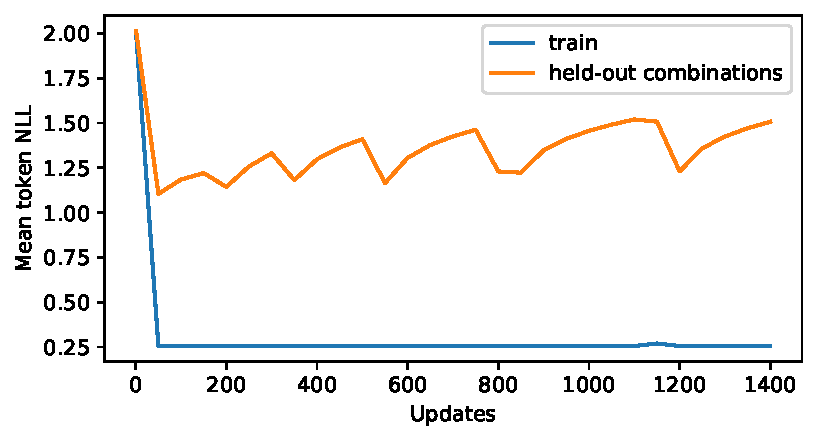
\includegraphics[width=.66\textwidth]{generated/language_model.pdf}
\caption{已有固定划分实验的训练与测试 token 损失. 局部叫声正确与整句预测质量是不同指标.}\label{fig:lm}
\end{figure}
同一前缀在训练中可能接不同颜色或主语, 所以最优训练损失也不为零. 对前缀 $c$, 训练后继频率为 $\widehat p(\cdot\mid c)$, 模型分布为 $q$, 则
\[
-\sum_y\widehat p_y\log q_y
=H(\widehat p)+\KL(\widehat p\Vert q)\ge H(\widehat p).
\]
按前缀出现次数加权, 得到这份经验训练资料的不可约下界, 约为 0.2560. 测试中的新组合可能不服从训练后继频率, 所以接近训练下界也不保证泛化. 两个测试样本、一个种子不足以证明稳定的组合能力. 翻转测试样本的中间动物恰好回到训练组合, 这个干预只能检验局部依赖, 不能作为新的组合留出.

\originalsection{上下文学习与条件任务推断}\label{sec:icl}
在预训练或后训练之后, 可以把任务示例放进提示:
``输入 1 输出 2; 输入 2 输出 4; 输入 3 输出?''
推理程序仍使用同一参数 $\theta$. 改变的是前缀 $c$, 于是改变 $p_\theta(y\mid c,x)$, 不是执行 $\theta\leftarrow\theta-\eta\nabla\mathcal L$. 本章把模型通过提示中的示例适应任务的行为称为上下文学习, 即 in-context learning, 简记 ICL. 它可在一次前向与后续生成中发生, 不要求任何优化器步骤. GPT-3 论文的摘要明确把 few-shot 示例置于文本交互中, 未在这些评价中更新模型权重\cite{gpt3}.

为什么不更新权重也能适应任务? 先研究一个真正可算的固定预测器. 假设隐藏任务 $h$ 只可能是 $h_0:y=x$ 与 $h_1:y=1-x$, 先验各为 $1/2$. 观察含噪示例时, 正确标签概率为 $0.9$, 翻转概率为 $0.1$, 各示例在给定任务后独立. 若两个示例都符合 $h_0$, 则 Bayes 公式给出
\[
P(h_0\mid c)=\frac{(1/2)0.9^2}{(1/2)0.9^2+(1/2)0.1^2}=\frac{81}{82}.
\]
对新输入 $x=1$, 标签为 1 的预测概率不是 $81/82$, 因为新标签仍含噪声, 而是 $(81\cdot0.9+1\cdot0.1)/82=73/82$. 先验与噪声规则都没有更新, 改变的是根据当前提示得到的任务后验. 因而 ``参数固定'' 与 ``行为能适应'' 并不矛盾.

首次阅读可先看随后的一维数字例, 再按需阅读一般矩阵形式. 向量、正定矩阵、谱与逆的工具见附录 \ref{ch:linear} 的表示空间与谱/SVD小节; 离散条件概率和期望见附录 \ref{ch:prob}. 本例额外调用如下明示的连续高斯密度与积分性质, 不要求把它们误当作此前已证明的内容. 下一例把离散任务推广到连续参数. 为避免把连续概率当作已学内容, 先约定: 密度 $f(w)$ 非负且积分为 1, 区域概率为在该区域上的积分, 条件密度仍由先验乘似然后归一化得到. 一维高斯密度为 $(2\pi\sigma^2)^{-1/2}\exp[-(w-\mu)^2/(2\sigma^2)]$, 均值为 $\mu$, 方差为 $\sigma^2$. 多维正定协方差 $\Sigma$ 的相应密度为
\[
(2\pi)^{-d/2}(\det\Sigma)^{-1/2}
\exp[-\tfrac12(w-\mu)^\top\Sigma^{-1}(w-\mu)].
\]
它的均值与协方差可由对称性、正交对角化和一维高斯积分核对. 本例使用这些高斯积分性质作为明确调用的工具, 核心工作是推导提示怎样改变后验与预测; 先复算随后的一维数字也能理解这一关系.

\begin{proposition}
设隐藏任务参数 $w\in\R^d$ 的先验密度与 $\exp(-\norm w^2/2)$ 成比例, 支持示例满足 $y=Xw+\varepsilon$, 其中 $X\in\R^{n\times d}$, $y\in\R^n$, 噪声向量 $\varepsilon$ 独立于 $w$, 各分量互相独立且为方差 $\sigma^2>0$ 的零均值高斯量. 令
\[
\Lambda=I_d+X^\top X/\sigma^2,\qquad
\mu=\Lambda^{-1}X^\top y/\sigma^2.
\]
任务后验为均值 $\mu$、协方差 $\Lambda^{-1}$ 的高斯分布. 对新输入 $x_*\in\R^d$, 新噪声 $\varepsilon_*$ 独立于 $w$ 和全部训练噪声, 且同为方差 $\sigma^2$ 的零均值高斯量. 标签预测均值为 $x_*^\top\mu$, 方差为 $\sigma^2+x_*^\top\Lambda^{-1}x_*$.
\end{proposition}
\begin{proof}
先验乘似然后取负对数, 与 $w$ 有关的部分为
\[
\tfrac12w^\top w+\tfrac1{2\sigma^2}(y-Xw)^\top(y-Xw)
=\tfrac12w^\top\Lambda w-w^\top X^\top y/\sigma^2+\text{常数}.
\]
$\Lambda$ 正定, 因为对非零 $v$, 有 $v^\top\Lambda v=\norm v^2+\norm{Xv}^2/\sigma^2>0$. 利用 $\Lambda\mu=X^\top y/\sigma^2$ 配方, 上式成为 $\tfrac12(w-\mu)^\top\Lambda(w-\mu)+\text{常数}$, 得到后验密度. 新噪声与 $w$ 独立, 所以 $y_*=x_*^\top w+\varepsilon_*$ 的均值与方差分别按线性期望和独立方差相加得到.
\end{proof}
一维时取 $X=(1,2)^\top,y=(2,4)^\top,\sigma^2=1$. 有 $\Lambda=6,\mu=10/6=5/3$. 查询 $x_*=3$, 预测均值为 5, 方差为 $1+9/6=2.5$. 无示例时先验均值为零, 预测方差为 $1+9=10$. 即使两点刚好共线, 有限噪声与先验收缩仍使预测均值不等于 6. \texttt{v03\_language.py} 的 \texttt{icl\_experiment} 按这个固定公式计算, 可训练权重更新次数为零.

这个例子说明了一种可能的任务推断机制, 没有证明 Transformer 都在执行这套 Bayes 计算. 隐式 Bayes 的相关论文提出了特定生成模型下的理论解释并报告受控实验\cite{iclbayes}; 其条件不是任意自然语言提示都满足的定理. 同样, 线性后验均值可以与正则化最小二乘得到同一数值, 也不说明模型内部真的运行梯度下降. 识别机制需要对任务分布、示例顺序、错误示例与查询作干预, 比较不同机制的预测, 而不是只看几个正确答案.

\originalsection{采样分布与序列决策}\label{sec:lm-sampling}
在每步 logits $z$ 上, 贪心解码取 $\arg\max_i z_i$. 它优化当前条件概率, 并不优化整条序列概率. 例如第一步 $p(a)=0.6,p(b)=0.4$, 接下来在 $a$ 后最好结束概率为 0.5, 在 $b$ 后结束概率为 1. 贪心路径概率为 $0.6\cdot0.5=0.3$, 另一条为 0.4. 比较序列概率时还要固定终止和长度处理, 不能把不同长度的分数随意混在一起.

温度采样把条件分布改为
\[
q_i(\tau)=\frac{\exp(z_i/\tau)}{\sum_j\exp(z_j/\tau)},\qquad\tau>0.
\]
有限词表下, $\tau\to\infty$ 时趋于均匀分布; $\tau\to0$ 时集中到最大 logit 集合, 若最大值并列则在它们之间均匀. 由 $q_i/q_j=e^{(z_i-z_j)/\tau}$ 可直接看出降温加强已有排序. 若排序最高的是错误答案, 降温会增加这种错误被选中的概率.

Top-$k$ 按概率排序保留前 $k$ 项后重归一化. Top-$p$ 先排序, 找累计概率首次达到阈值 $p\in(0,1]$ 的最短前缀, 保留它再归一化. 必须包含使累计概率越过阈值的那一项, 否则可能保留空集合. 并列项需要确定的排序规则. 同时使用两者时还要说明顺序: 新实验先应用 $k$, 在所剩分布上归一化, 再应用 $p$.

若原分布为 $(0.4,0.3,0.2,0.1)$, 温度 $1/2$ 相当于平方后归一化, 得 $(16,9,4,1)/30$. 阈值 $p=0.65$ 保留前两项, 得 $(4/7,3/7,0,0)$. 两者并不相同: 降温仍保留全部支持, 截断直接排除候选. 固定种子 144 下每种设置抽样 50,000 次, $p=0.65$ 的前两项实测频率为 0.56906 与 0.43094, 可与上述精确概率比较. 这检验采样实现, 没有包含答案真伪标签.

\originalsection{KV 缓存的等价性与成本}\label{sec:lm-cache}
生成新 token 前, 先处理整段提示, 称为 prefill; 此后逐 token 推进, 称为 decode. 不缓存时, 可在每轮对完整前缀重新运行网络. 因果结构使大量旧计算保持不变, 所以可以复用.

\begin{proposition}\label{prop:kv-equivalence}
固定参数、位置编号与前缀, 在评价模式下使用确定的逐位置前馈运算与因果注意力. 每层缓存旧位置的键和值, 新位置只计算自身隐藏状态、查询、键和值, 得到的末位置 logits 与重新计算完整前缀相同, 在实数精确运算意义下成立.
\end{proposition}
\begin{proof}
先对层数归纳. 输入层中, 旧位置的 token 与位置嵌入没有改变. 假定一层输入在旧位置保持不变, 则它们的键和值也不变. 旧位置的因果注意力只读取不晚于自身的位置, 所以新增位置不会影响它们; 逐位置残差、归一化与前馈网络亦不受影响. 对新位置, 缓存给出了完整前向中全部旧键值, 其自身的新键值也按同一输入计算. 相同查询与全部可见键产生相同注意力权重, 因而新位置输出一致. 此论证逐层成立, 最终逐位置输出映射也一致.
\end{proof}
这个条件排除了重新编号旧位置、修改前缀、丢弃部分缓存、随机 dropout 等情形. 采用旋转位置编码时, 也应在写入键缓存时使用正确绝对位置或等价的相对位置约定. 量化缓存会引入数值近似, 不能仍宣称与未量化的完整前向严格相同. 实数等价也不要求不同矩阵计算顺序在浮点中逐位一致.

单层单头当前长度 $t$ 的新查询形状为 $B\times1\times d$, 缓存键值均为 $B\times t\times d$, 分数形状为 $B\times1\times t$. 一轮的键查询与加权值乘积成本为 $O(Btd)$, 新位置线性投影与前馈成本约为 $O(Bd^2)$, 输出词表投影为 $O(BdV)$. 对 $L$ 层的多头模型, 若键值各头总宽度为 $d_{\rm KV}$, 长度为 $t$, 缓存元素为 $2BLtd_{\rm KV}$. 每元素占 $s$ 字节时, 主体内存为 $2BLtd_{\rm KV}s$, 未计元数据与临时激活. 分组查询让多个查询头共享键值头, 可以减小 $d_{\rm KV}$.

从空前缀依次生成 $T$ 个输入位置时, 缓存注意力总成本为 $O(LBT^2d)$, 新位置投影总成本为 $O(LBTd^2)$. 若每轮重新计算完整前缀, 注意力成本为 $O(LB\sum_{t=1}^Tt^2d)=O(LBT^3d)$, 投影为 $O(LBT^2d^2)$. 这描述特定重复前向实现的算术量, 不表示所有解码系统的墙钟时间按这个比率改善. 当输出投影、缓存读带宽或小矩阵调度占主导时, 瓶颈不同.

新实验复用 \texttt{TinyDecoder} 的固定参数, 独立实现 \texttt{CachedDecoder.step}. 对 $B=3,T=12,d=8,V=10$, 比较全部十二个前缀的末位置 logits, 最大绝对差为 $2.22\times10^{-16}$. 修改最后 token 对旧位置 logits 的最大影响为零. 缓存共 576 个数. 重新计算完整分数矩阵的槽位总数为 $3\sum_{t=1}^{12}t^2=1950$, 增量计算为 $3\sum_{t=1}^{12}t=234$; 这是可核对的计数, 没有冒充测速结果.

\originalsection{复算与练习}
新增实验的统一入口为 \texttt{experiments/v03\_language.py}, 只使用 NumPy、原创有限资料与旧小模型参数接口. 运行命令为
\begin{center}\texttt{PYTHONDONTWRITEBYTECODE=1 python experiments/v03\_language.py --seed 144}\end{center}
结果保存在 \path{results/v03-language/metrics.json}, 环境、参数来源哈希与种子保存在同目录的 \path{environment.json}. 该命令不训练或下载外部语言模型. 实验中的数学等价性由前面证明支持, 数值运行用于发现实现偏差; 误差容限与七项机制测试见 \path{tests/test_v03_language.py}.

\begin{exercise}
用 2 个有效 token 的小批和 6 个有效 token 的小批累计梯度, 两个按 token 平均的梯度分别是 $g_1,g_2$. 写出大批梯度. 若先平均二者再把学习率调整一个常数, 能否对任意 $g_1,g_2$ 恢复它?
\end{exercise}
\begin{solution}
正确梯度为 $g_1/4+3g_2/4$. 直接平均给 $(g_1+g_2)/2$. 若只乘常数 $c$, 需要同时 $c/2=1/4$ 与 $c/2=3/4$, 不可能. 问题是样本权重改变, 不是统一梯度尺度改变.
\end{solution}
\begin{exercise}
二元任务算例中, 两个示例一个符合 $h_0$, 一个符合 $h_1$. 后验如何? 若模型得到同样答案, 是否足以认定它内部使用 Bayes 推断?
\end{exercise}
\begin{solution}
两个任务的似然均为 $0.9\cdot0.1$, 后验仍各为 $1/2$, 新标签预测也各为 $1/2$. 同一输出可能由查表、计数规则或 Bayes 推断实现. 应设计多种示例数量、噪声与先验条件, 检查各候选机制的不同预测; 有限成功仍不能唯一确定内部算法.
\end{solution}
\label{ch:end:prediction}
